\section{Introduction}
\par The development of numerical solver that solves the lid driven cavity
flow problem on a square domain of side 2 meters was performed in the present
work. Air under standard atmospheric conditions was chosen as the working
fluid and the computation was perfomed using finite-difference method.\\

\par The analysis was supposed to be performed on a colocated grid with
fractional step method, but the method was found to be stiff and requiring
quite more time to fix, hence the present work was done using the staggered-grid
pressure correction technique and SIMPLE algorithm. \cite{ref_1} is used as the
reference for the computation procedure.

\section{Computation procedure}
\par The 2D incompressible Navier-Stokes equations were solved in the present
work in the partial differential form as given in \Cref{ns_eqn1,ns_eqn2,ns_eqn3}.
\begin{align}
    \frac{\partial u}{\partial x} + \frac{\partial v}{\partial y} &= 0 \label{ns_eqn1} \\
    \frac{\partial u}{\partial t} + u\frac{\partial u}{\partial x} + v\frac{\partial u}{\partial y} &= -\frac{1}{\rho}\frac{\partial p}{\partial x} + \nu \left(\frac{\partial^2 u}{\partial x^2} + \frac{\partial^2 u}{\partial y^2}\right) \label{ns_eqn2} \\
    \frac{\partial v}{\partial t} + u\frac{\partial v}{\partial x} + v\frac{\partial v}{\partial y} &= -\frac{1}{\rho}\frac{\partial p}{\partial x} + \nu \left(\frac{\partial^2 v}{\partial x^2} + \frac{\partial^2 v}{\partial y^2}\right) \label{ns_eqn3}
\end{align}

\par The computation was performed on a \emph{forward staggered grid}, i.e. the
staggered grid with pressure nodes covering the boundaries and velocity nodes
present between them at equal spaces. The schematic of the domain is shown
in \Cref{staggered_grid}.
\begin{figure}
   \centering
    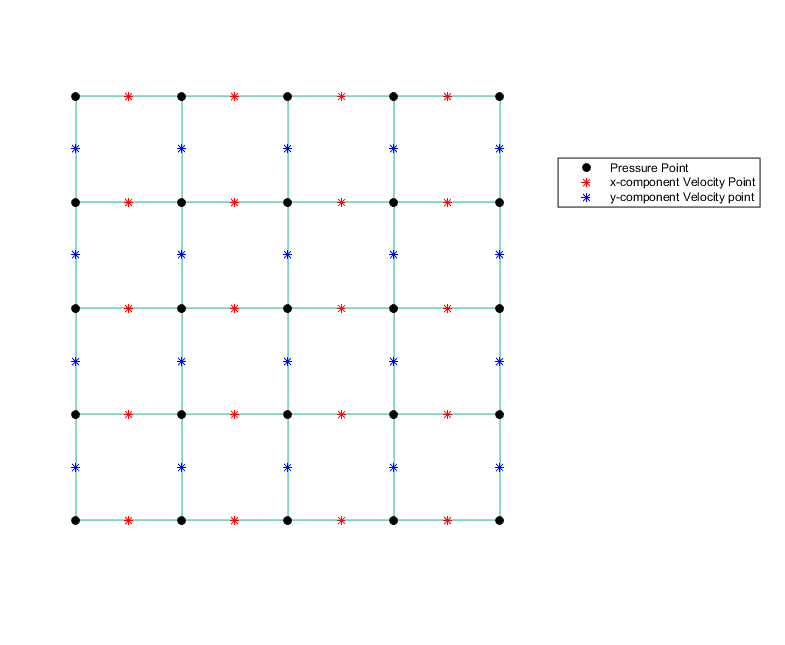
\includegraphics[scale=0.5]{supporting_documents/staggered_grid_5X5.png}
    \caption{forward staggered grid arrangement}
    \label{staggered_grid}
\end{figure}

\par Then the equations are discretized with finite difference technique using
central difference for all the spacial derivatives and forward difference for
the temporal derivative. The discretized and rearranged momentum equations
are given in \Cref{x_mmtm_discretized,y_mmtm_discretized}

\begin{align}
    u_{i,j}^{n+1} &= u_{i,j}^{n} + \Delta t \left(-F_{term} + D_{term} - P_{term}\right) \label{x_mmtm_discretized} \\
    \text{where,} \nonumber \\
    F_{term} &= \frac{u_{i+1,j}^2 - u_{i-1,j}^2}{2 dx} + \frac{uv_{i,j+1} - uv_{i,j-1}}{2 dy} \nonumber \\
    D_{term} & = \nu \left(\frac{u_{i+1,j} - 2 u_{i,j} + u_{i-1,j}}{dx^2} + \frac{u_{i,j+1} - 2 u{i,j} + u{i,j-1}}{dy^2}\right) \nonumber \\
    P_{term} &= \frac{1}{\rho}\frac{p_{i+1,j} - p_{i-1,j}}{2 dx} \nonumber
\end{align}

\begin{align}
    v_{i,j}^{n+1} &= v_{i,j}^{n} + \Delta t \left(-F_{term} + D_{term} - P_{term}\right) \label{y_mmtm_discretized} \\
    \text{where,} \nonumber \\
    F_{term} &= \frac{uv_{i+1,j} - uv_{i-1,j}}{2 dx} + \frac{v_{i,j+1}^2 - v_{i,j-1}^2}{2 dy} \nonumber \\
    D_{term} & = \nu \left(\frac{v_{i+1,j} - 2 v_{i,j} + v_{i-1,j}}{dx^2} + \frac{v_{i,j+1} - 2 v{i,j} + v{i,j-1}}{dy^2}\right) \nonumber \\
    P_{term} &= \frac{1}{\rho}\frac{p_{i,j+1} - p_{i,j-1}}{2 dy} \nonumber
\end{align}

\par The pressure correction equation was derived as given in \cite{ref_1} and
is given as \Cref{pp_eqn}
\begin{align}
    a p^{\prime}_{i,j} + b (p^{\prime}_{i+1,j}  + p^{\prime}_{i-1,j}) + c (p^{\prime}_{i,j+1} + p^{\prime}_{i,j-1}) + d = 0 \label{pp_eqn}
\end{align}

\par where, the coefficients are as given below.
\begin{align*}
    a &= \left(\frac{2 dt}{dx^2} + \frac{2 dt}{dy^2}\right) \\
    b &= - \frac{dt}{dx^2} \\
    c &= - \frac{dt}{dy^2} \\
    d_{i,j} &= \frac{1}{dx}\left(\rho u^*_{i,j} - \rho u^*_{i-1,j}\right) + \frac{1}{dy} \left(\rho v^*_{i,j} -\rho v^*_{i,j-1}\right)
\end{align*}

\par further the computed pressure correction field \(p^{\prime}\) is used to
correct the pressure and velocity as given in \Cref{p_cor_eqn,u_cor_eqn,v_cor_eqn}.
\begin{align}
    p_{i,j} &= p_{i,j}^* + \alpha p_{i,j}^{\prime} \label{p_cor_eqn} \\
    u_{i,j} &= u_{i,j}^* - \alpha \left.\frac{\partial p^{\prime}}{\partial x}\right\vert_{i,j} \label{u_cor_eqn} \\
    v_{i,j} &= v_{i,j}^* - \alpha \left.\frac{\partial p^{\prime}}{\partial y}\right\vert_{i,j} \label{v_cor_eqn}
\end{align}

\par where, \(\alpha = 0.1 \) is the under-relaxation factor used in the present
computation work.\\

\par It is to be noted that there will be three overlapping grids, each for each
flow field variable \emph{u,v,p}, hence in the code, the indexing was taken care
such that the velocity at a given point is driven by the pressure nodes surrounding
it. This has to be taken care on doing coding. \\

\par The SIMPLE (Semi-Implicit Method for Pressure Linked Equations) algorithm
was implemented for the computation of solution fields. The steps followed are
as follows.
\begin{enumerate}
    \item Initial pressure field was assumed and \Cref{x_mmtm_discretized,y_mmtm_discretized} were
        solved for an intermediate velocity field which is called as \(u^*, v^*\).
    \item Then the mass imbalance term \emph{d} in \Cref{pp_eqn} was computed then the pressure
        correction field \(p^{\prime}\) was computed.
    \item The computed pressure correction field was then used to update the
        pressure and velocity field using \Cref{p_cor_eqn,u_cor_eqn,v_cor_eqn}.
    \item The above procedure is repeated till the solution converges, i.e. the
        mass imbalance term \(d \rightarrow 0\).
\end{enumerate}

\par Since, this is a driven cavity flow problem, the generation of flow
vorticity will be significant and it would be better to visualize the results
in terms of the vorticity contour. Hence the \Cref{vorticity_eqn} is used to
compute the vorticity term during post-processing.
\begin{align}
    \omega = \frac{\partial u}{\partial y} - \frac{\partial v}{\partial x} \label{vorticity_eqn}
\end{align}

\pagebreak

\section{Results}
\par The simulation was carried out for 300 seconds to study how the flow pattern
emerges with time. The intermediate timestep solution fields were saved to
csv files and were used in post-processing to generate animations of solution
fields with time. The several contours obtained at different time steps and are
shown in \Cref{vorticity_streamlines_contour,velocityMagnitude_contour}.


\begin{figure}[!h]
    \begin{subfigure}{0.5\textwidth}
       \centering
        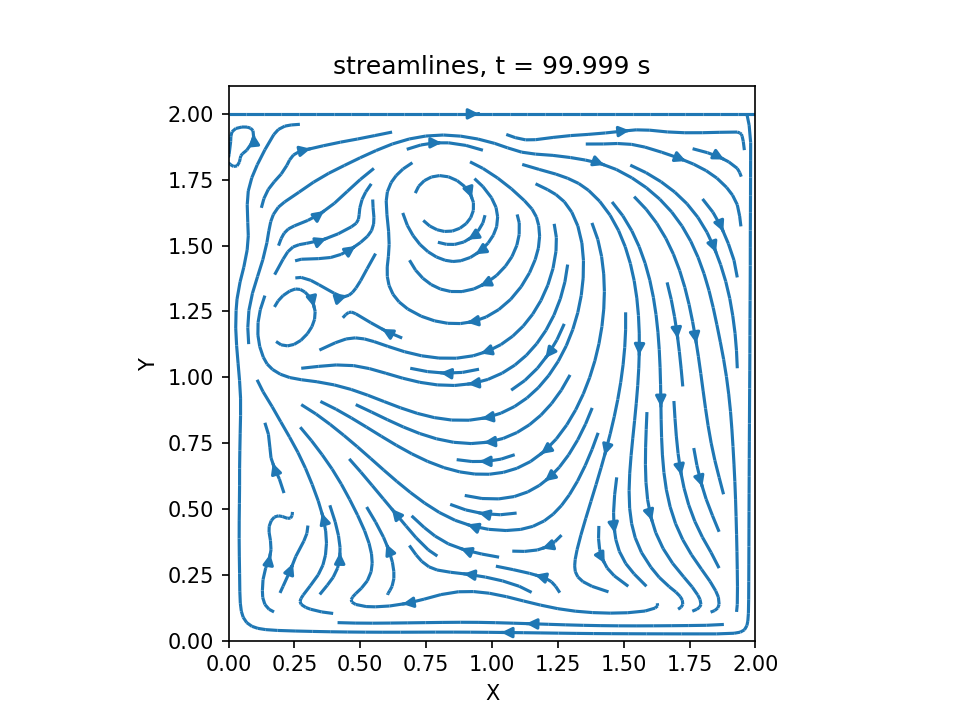
\includegraphics[scale =0.5]{supporting_documents/contours/streamlines/streamlines_0000000100.png}
        \caption{streamline pattern, t = 100 s}
    \end{subfigure}
   \hfill
    \begin{subfigure}{0.5\textwidth}
       \centering
        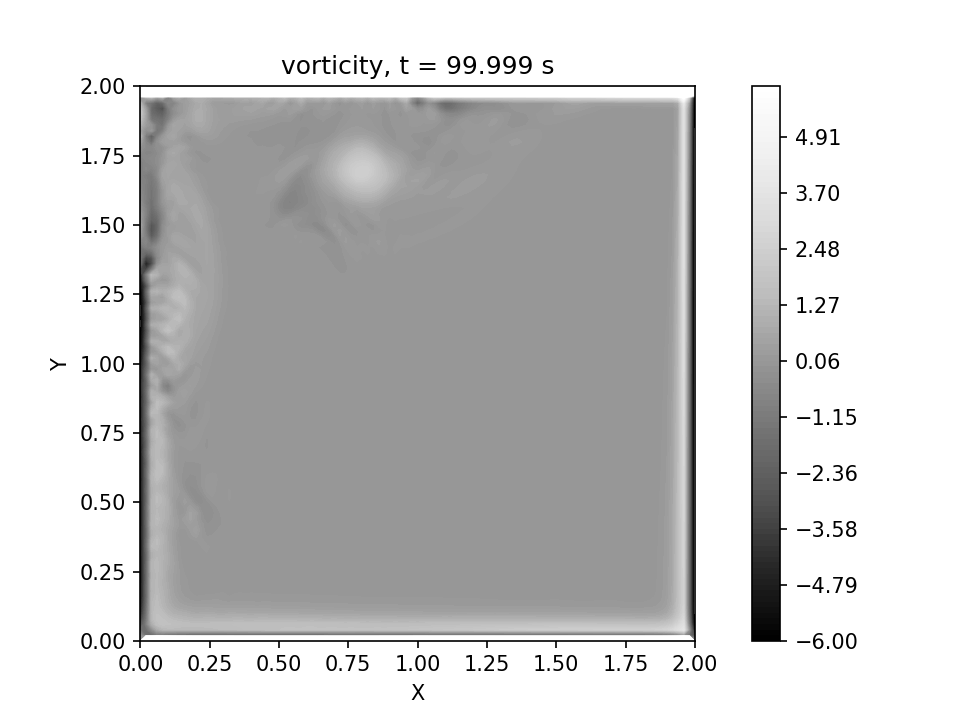
\includegraphics[scale =0.5]{supporting_documents/contours/vorticity/vorticity_0000000100.png}
        \caption{vorticity, t = 100 s}
    \end{subfigure}
   \hfill
    \begin{subfigure}{0.5\textwidth}
       \centering
        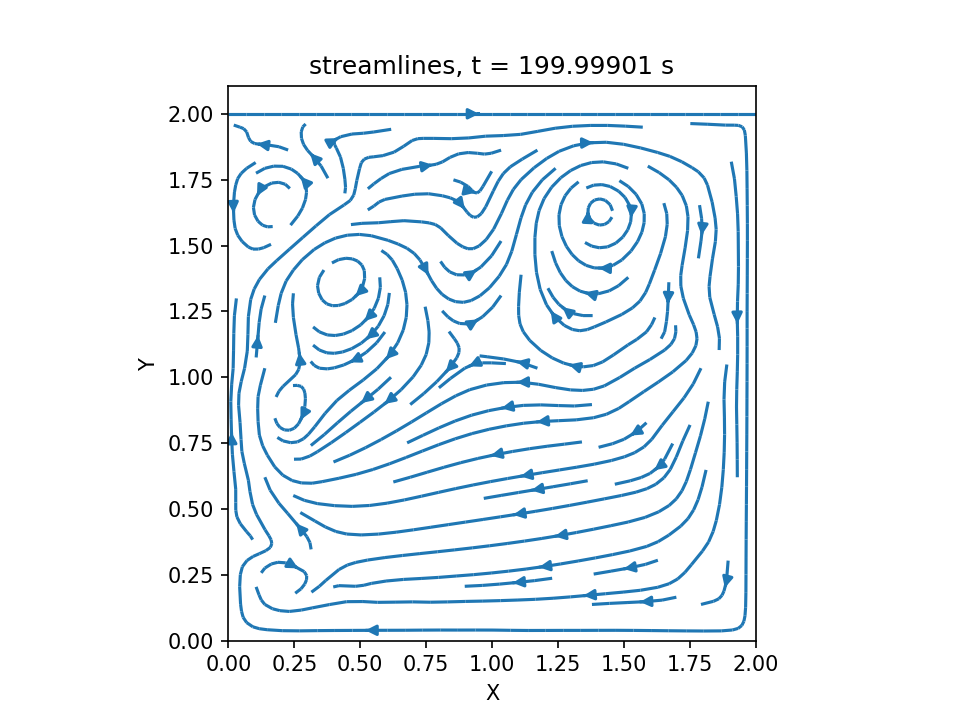
\includegraphics[scale =0.5]{supporting_documents/contours/streamlines/streamlines_0000000200.png}
        \caption{streamline pattern, t = 200 s}
    \end{subfigure}
   \hfill
    \begin{subfigure}{0.5\textwidth}
       \centering
        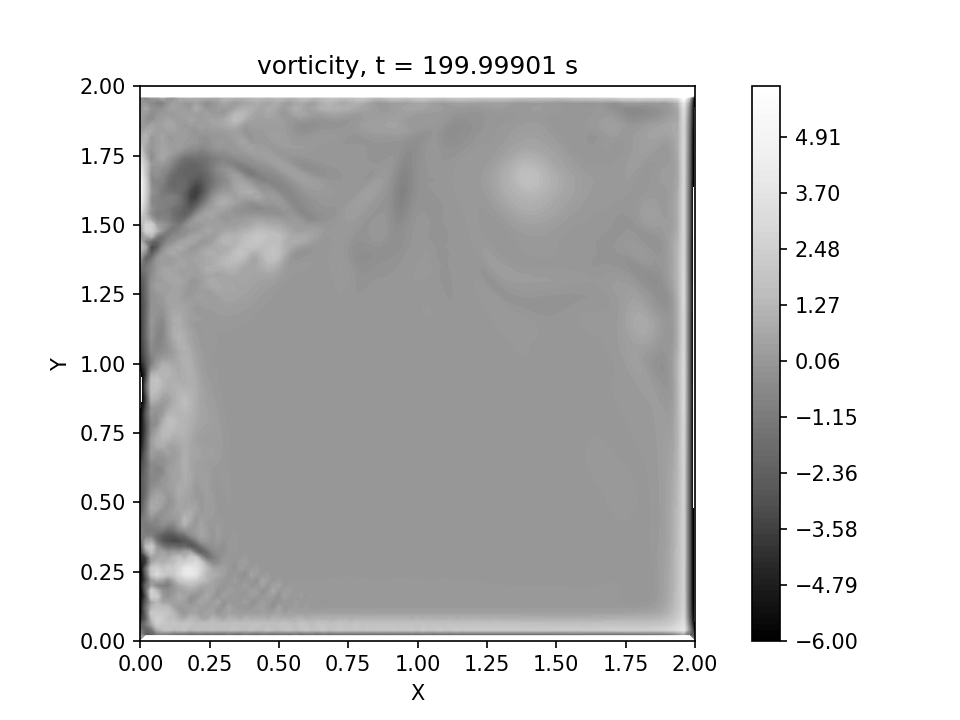
\includegraphics[scale =0.5]{supporting_documents/contours/vorticity/vorticity_0000000200.png}
        \caption{vorticity, t = 200 s}
    \end{subfigure}
\end{figure}
\begin{figure}
   \continuedfloat
    \begin{subfigure}{0.5\textwidth}
       \centering
        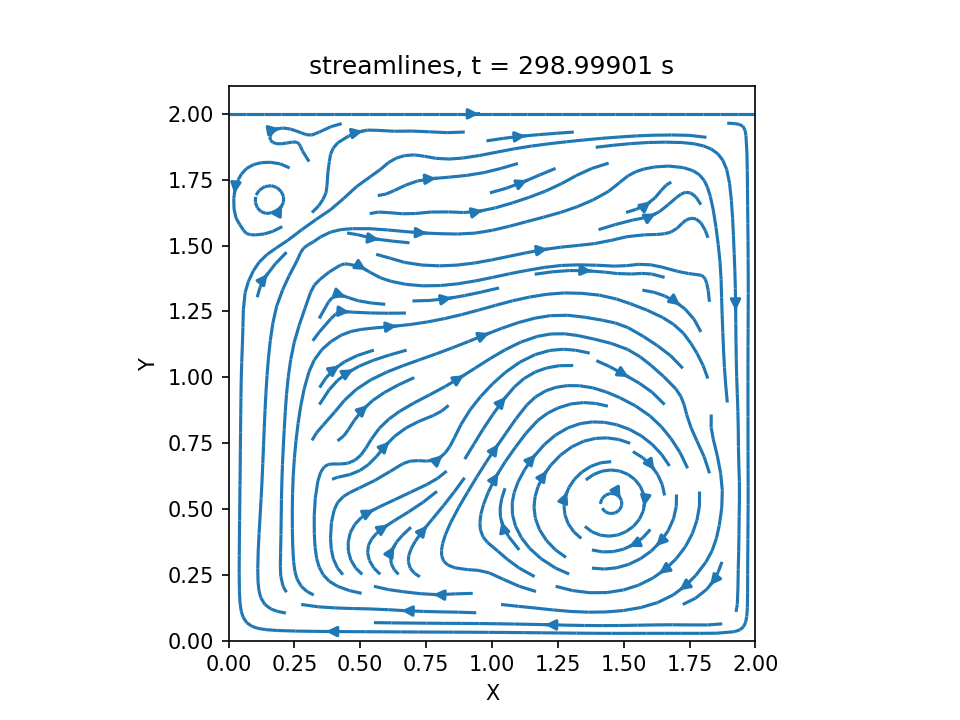
\includegraphics[scale =0.5]{supporting_documents/contours/streamlines/streamlines_0000000299.png}
        \caption{streamline pattern, t = 299 s}
    \end{subfigure}
   \hfill
    \begin{subfigure}{0.5\textwidth}
       \centering
        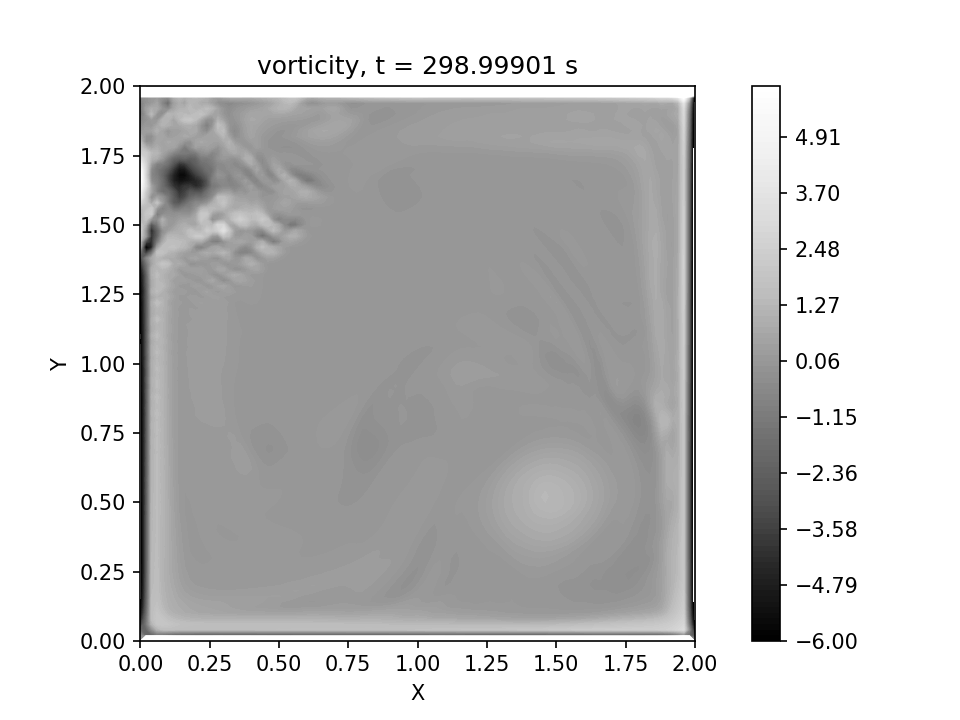
\includegraphics[scale =0.5]{supporting_documents/contours/vorticity/vorticity_0000000299.png}
        \caption{vorticity, t = 299 s}
    \end{subfigure}
    \caption{vorticity and streamlines patterns at different solution timesteps}
    \label{vorticity_streamlines_contour}
\end{figure}

\pagebreak


\begin{figure}

    \begin{subfigure}{0.5\textwidth}
       \centering
        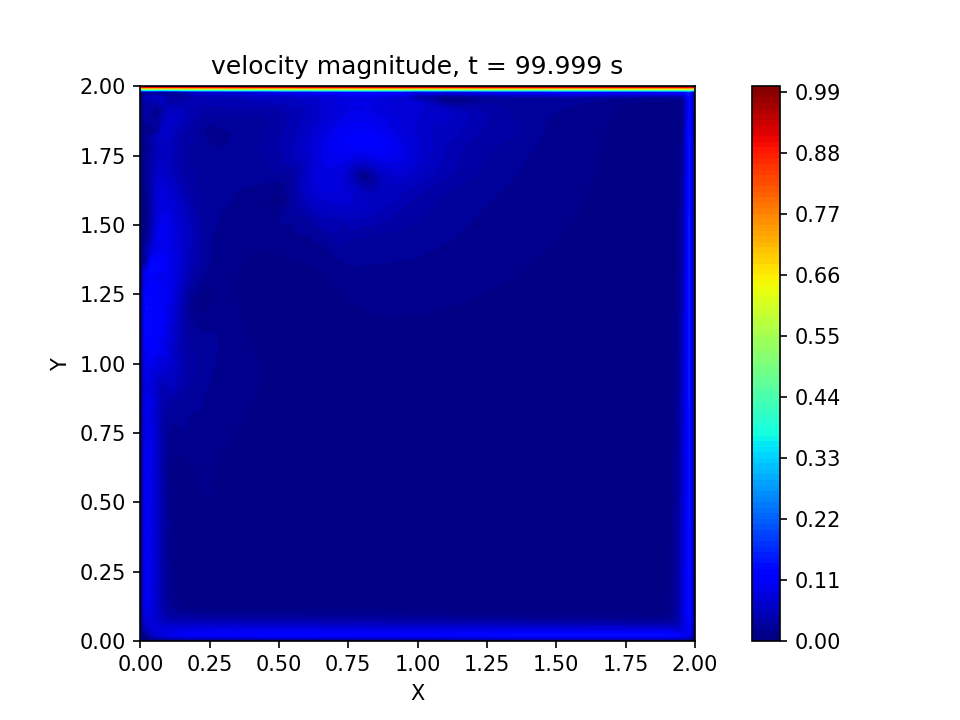
\includegraphics[scale=0.5]{supporting_documents/contours/velocity-magnitude/velocityMagnitude_0000000100.png}
        \caption{velocity magnitude, t = 100s}
    \end{subfigure}
    \hfill
    \begin{subfigure}{0.5\textwidth}
       \centering
        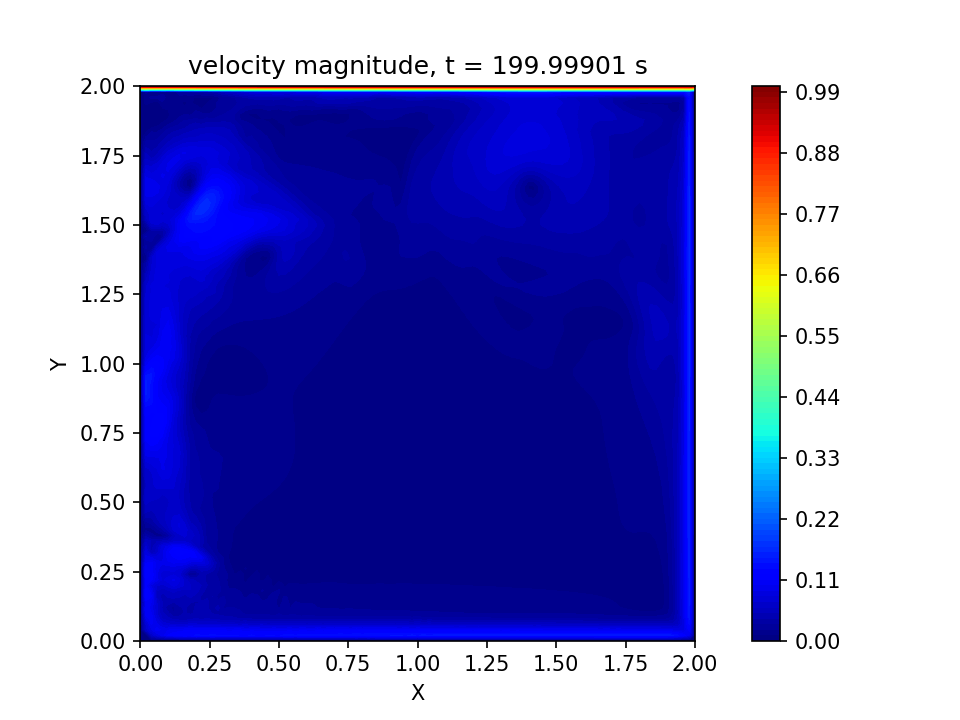
\includegraphics[scale=0.5]{supporting_documents/contours/velocity-magnitude/velocityMagnitude_0000000200.png}
        \caption{velocity magnitude, t = 200s}
    \end{subfigure}
    \hfill
    \begin{subfigure}{1\textwidth}
       \centering
        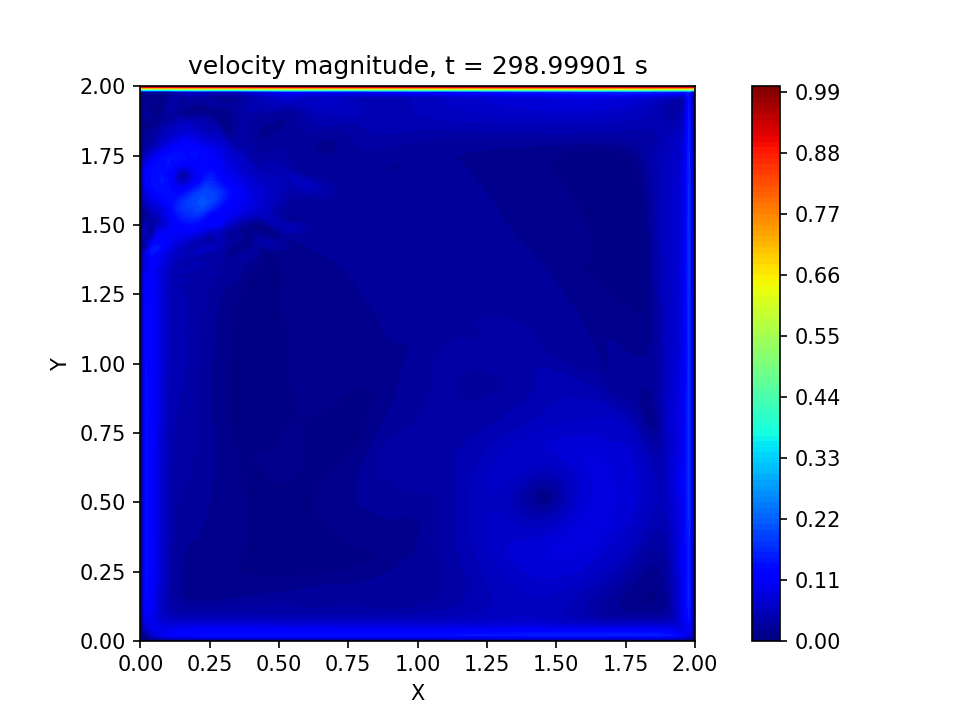
\includegraphics[scale=0.5]{supporting_documents/contours/velocity-magnitude/velocityMagnitude_0000000299.png}
        \caption{velocity magnitude, t = 299s}
    \end{subfigure}

    \caption{velocity magnitude contours at different simulation times}
    \label{velocityMagnitude_contour}

\end{figure}

\pagebreak

\section{Conclusion and further works}
\par The numerical computation of lid driven cavity flow problem for the given
configuration was successfully performed using staggered-grid finite difference
method and pressure correction technique, SIMPLE algorithm. The further work
will be based on the investigation on why the fractional step method did not
work and the development of the code based on fractional step method that
solves the same problem. The codes developed for this assignment are given in
\Cref{numerical_code}.
